\chapter{Desenvolvimento}
\label{chapter:desenvolvimento}

Neste capítulo, são apresentadas a contribuição deste trabalho. Na Seção \ref{sec:metodologia} é apresentada a metodologia utilizada para a coleta e processamento dos dados. Na Seção \ref{sec:resultados} são apresentados os resultados encontrados na abordagem.

\section{Metodologia Utilizada} \label{sec:metodologia}

%Foi planejado e realizado um estudo que visa avaliar estado manutenibilidade
%do Linux Kernel, utilizando o sofware SonarQube para a medição. Os
%requerimentos necessários pelo método SQALE foram as fornecidas pelo
%plugin \textbf{sonar-cxx\cite{Sonarcxx2016}}. O software realiza
%uma leitura completa do código fonte da aplicação a ser analisada,
%identificando os trechos não adequados de acordo com os requerimentos
%definidos. Para cada não conformidade encontrada, há uma função de
%remediação definida com o tempo estimado de remediação cada ocorrência
%encontrada. Foram consideradas 6 versões de lançamento estáveis foram
%analisadas dentro das versões mais recentes, procurando avaliar o
%estado atual da manutenibilidade do software. 

Nesta seção, é apresentada a metodologia utilizada para coleta e análise dos dados. Foram utilizamos os repositórios da \textit{Apache Software Foundation}, onde o código fonte dos \textit{softwares} é armazenado, através do sistema de controle de versão \textit{Git}\footnote{Disponível em https://git-scm.com/}. O \textit{software Git} permite que configurações do projeto(código fonte, arquivos de configuração, artefatos) sejam salvos(em \textit{commits}), mantendo um histórico do estado de todo o projeto ao longo da sua evolução. 

Nele, marcações (\textit{tags}) podem ser criadas para referenciar uma determinada versão. Tais marcações são utilizadas para sinalizar versões de lançamento. Para descrever a evolução do software, um número de versão é geralmente utilizado, contendo três componentes: versão principal(\textit{major version}), versão secundária(\textit{minor version}) e versão de manutenção, separados por pontos (ex: 1.0.0). Foram analisadas todas as versões marcadas como lançamentos em que o número da versão não fosse inferior ao atual, evitando assim que as análises fossem realizadas em versões de manutenção, que possuem evolução paralela. Um simples exemplo é apresentado na figura \ref{fig:selecaoversoes}.
\begin{figure}[h]
	\centering
	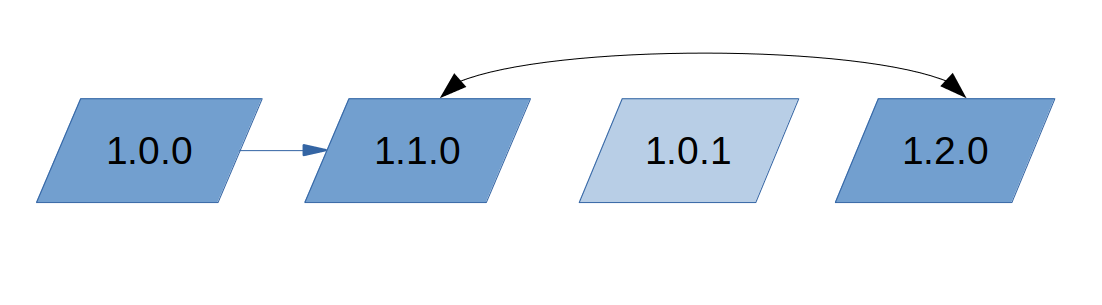
\includegraphics[width=0.7\linewidth]{figure/selecao_versoes}
	\caption{}
	\label{fig:selecaoversoes}
\end{figure}

As métricas mostradas são apresentadas como uma função do tempo, devido a grande variância de lançamento de versões menores. Por exemplo, uma versão nomeada "2.1.1" pode ser lançada após o lançamento de uma versão "3.0.0". Portanto, utilizar as métricas como funções de números de versões pode levar a resultados enganosos, assim como descrito e adotado em \cite{israeli2010linux}.

A descrição de cada métrica utilizada é apresentada em conjunto com sua observação, descritas na seção seguinte.
\section{Resultados} \label{sec:resultados}

Nesta seção analisamos as Leis de Evolução de Software de Lehman, assim como apresentadas na Seção \ref{sec:lehmalaws} usando como base dados obtidos do \textit{Apache Hadoop}. Para cada lei, foram formuladas hipóteses para serem verificadas diante dos dados obtidos, assim como definidas em \cite{neamtiu2013towards}.

\subsection{Lei 1: Mudança Contínua}
Esta Lei determina que o software deve se adaptar constantemente, caso contrário torna-se obsoleto. Os projetos analisados são ativamente mantidos e largamente utilizados, portanto, se a lei é valida, deve-se observar que o programa está em constante mudança. Para caracterizar mudança, foi utilizado o número de adições e remoções em linhas de código do projeto. 
\begin{hypothesis}
	O número de mudanças cumulativas em cada release é diferente de zero.
\end{hypothesis}
\begin{figure}[h]
	\centering
	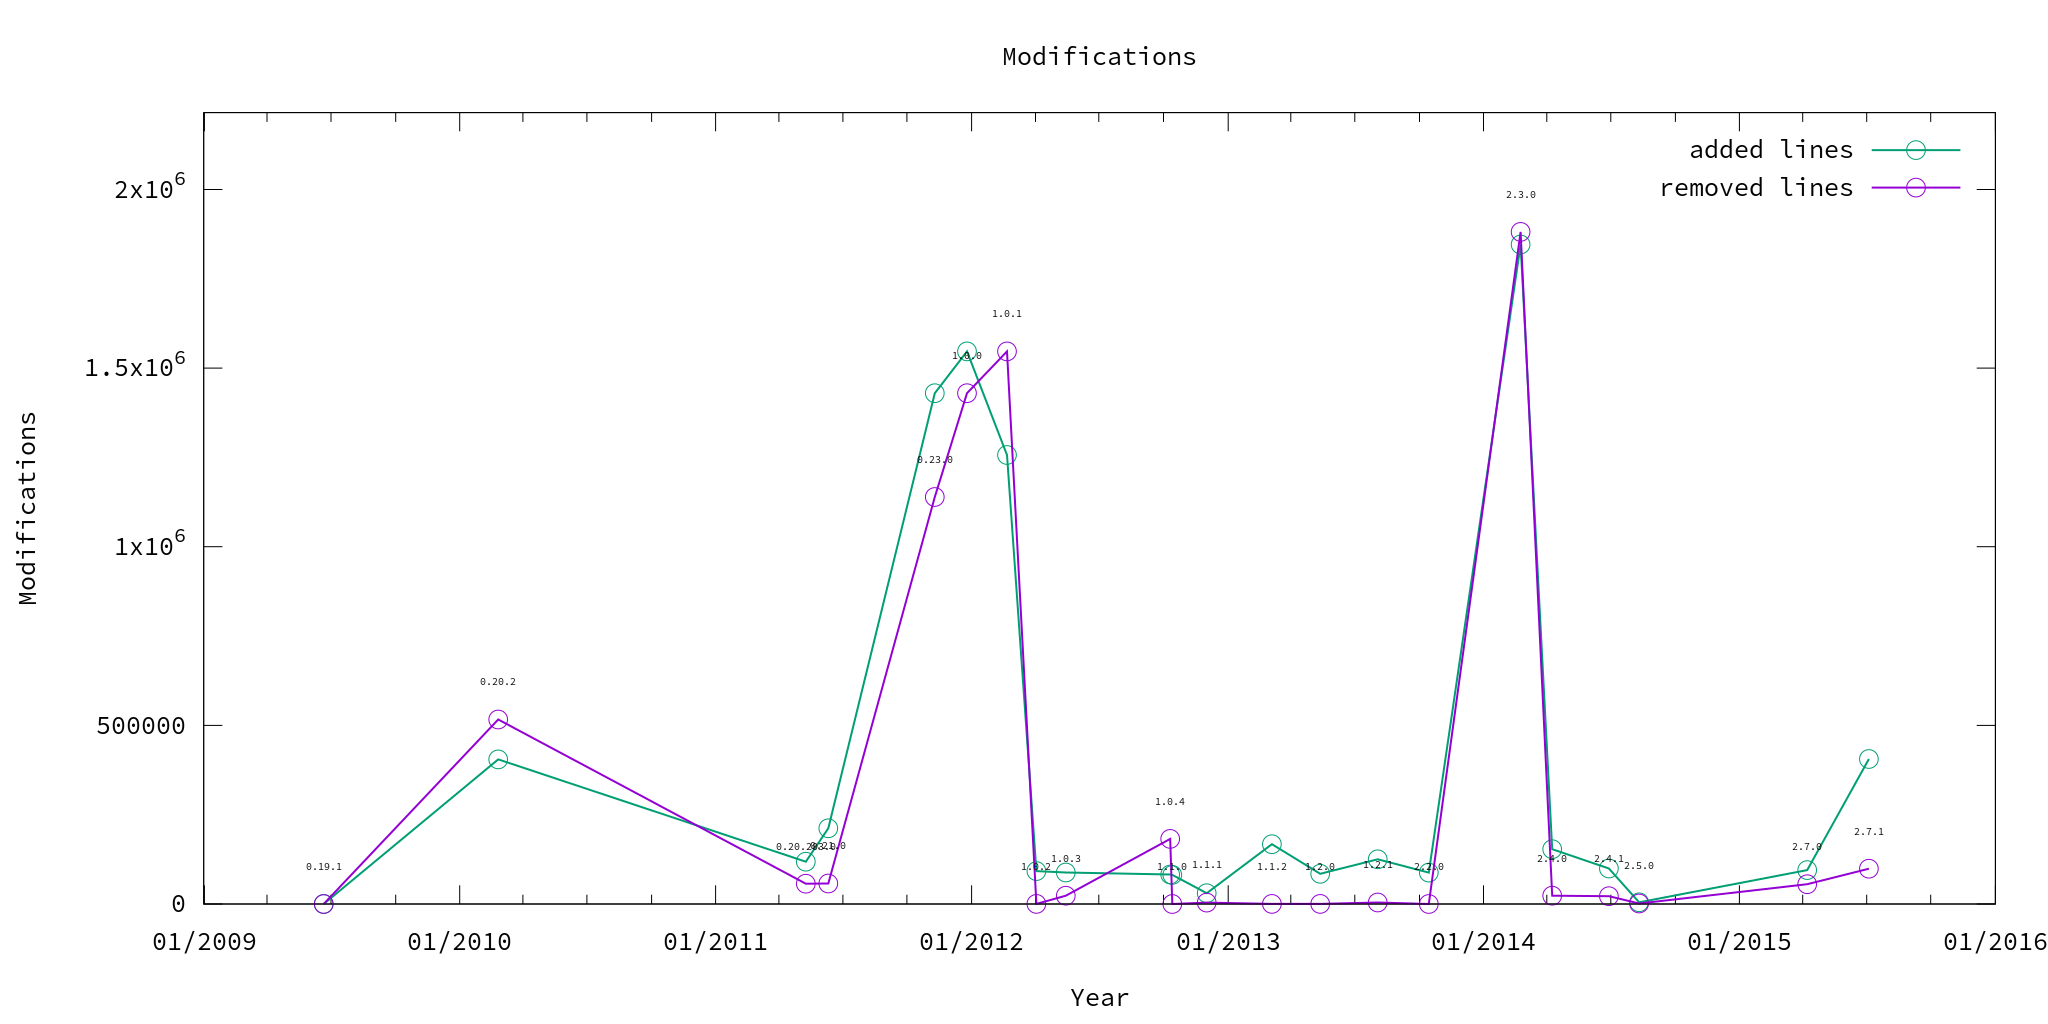
\includegraphics[width=0.9\linewidth]{figure/Modifications}
	\caption{Mudanças no software ao longo do tempo}
	\label{fig:modifications}
\end{figure}
O gráfico da figura \ref{fig:modifications} mostra a evolução das adições e remoções de linhas no projeto. Linhas que foram modificadas, são contabilizadas como uma remoção e uma adição. Notam-se grandes picos de mudanças quando o número de versão principal é alterado, em geral atribuído a adição de novos recursos ao \textit{software} ou restruturação de grandes partes do mesmo. Observa-se que salvo alguns pontos, o número de linhas adicionadas é superior ao de linhas removidas, o que é esperado se o projeto tende a incorporar novas funcionalidades.

Portanto, verifica-se que a primeira Lei de Lehman é confirmada para o \textit{Hadoop}.

\subsection{Lei 2: Complexidade Crescente}
A segunda lei postula que a medida que um programa cresce, sua complexidade aumenta se não forem realizadas medidas para prevenir tal fato. Para medição da complexidade do código, foi utilizada como métrica a complexidade ciclomática, assim como definido na Seção \ref{subsec:complexidade_ciclomatica}, como utilizado em estudos anteriores \cite{israeli2010linux,neamtiu2013towards,skoulis2014open}.
Foram tomadas as seguintes hipóteses:
\begin{hypothesis}
	A complexidade ciclomática total aumenta com o tempo.
\end{hypothesis}
\begin{hypothesis}
	A complexidade ciclomática relativa aumenta com o tempo.
\end{hypothesis}

Como a complexidade total do projeto é afetada pelo seu tamanho, precisamos avaliar também se a complexidade relativa do código cresce ao longo do tempo, isto é, se novas adições tendem a aumentar a complexidade do código em relação ao seu tamanho. A Figura \ref{fig:total_complexity} apresenta a complexidade ciclomática total do código, enquanto as Figuras \ref{fig:file_complexity},\ref{fig:functioncomplexity},\ref{fig:classcomplexity} mostram respectivamente a complexidade relativa número de arquivos, número de funções e número do de classes do projeto.
\begin{figure}[h]
	\centering
	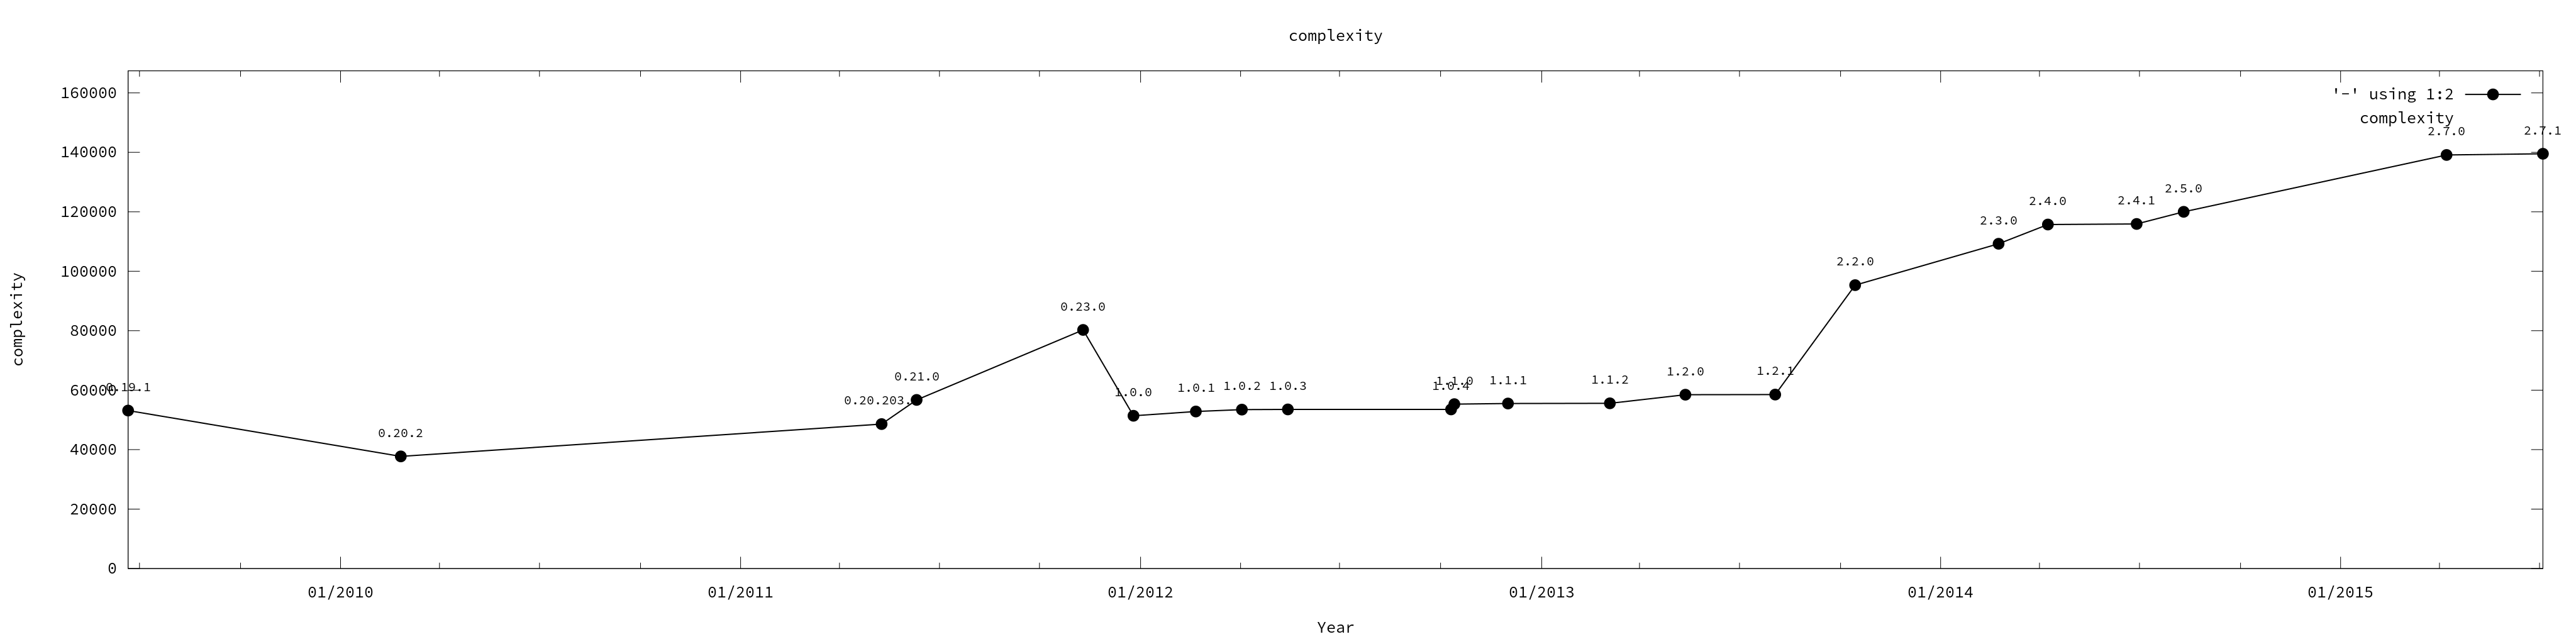
\includegraphics[width=0.9\linewidth]{figure/complexity}
	\caption{Evolução da Complexidade Ciclomática Total}
	\label{fig:total_complexity}
\end{figure}
\begin{figure}[h]
	\centering
	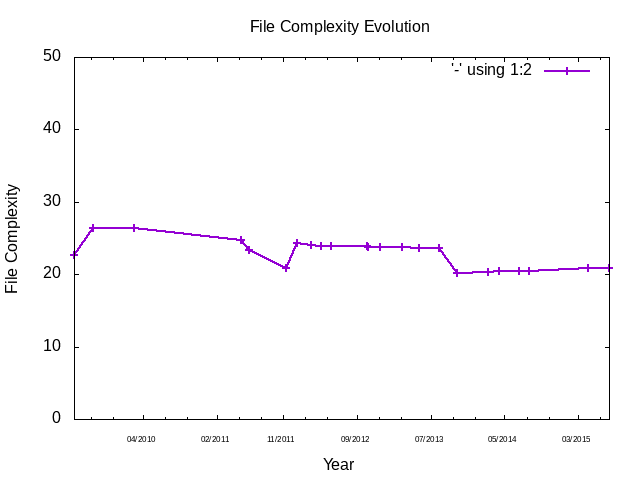
\includegraphics[width=1\linewidth]{figure/file_complexity}
	\caption{Evolução da complexidade/Arquivo}
	\label{fig:file_complexity}
\end{figure}
\begin{figure}[h]
	\centering
	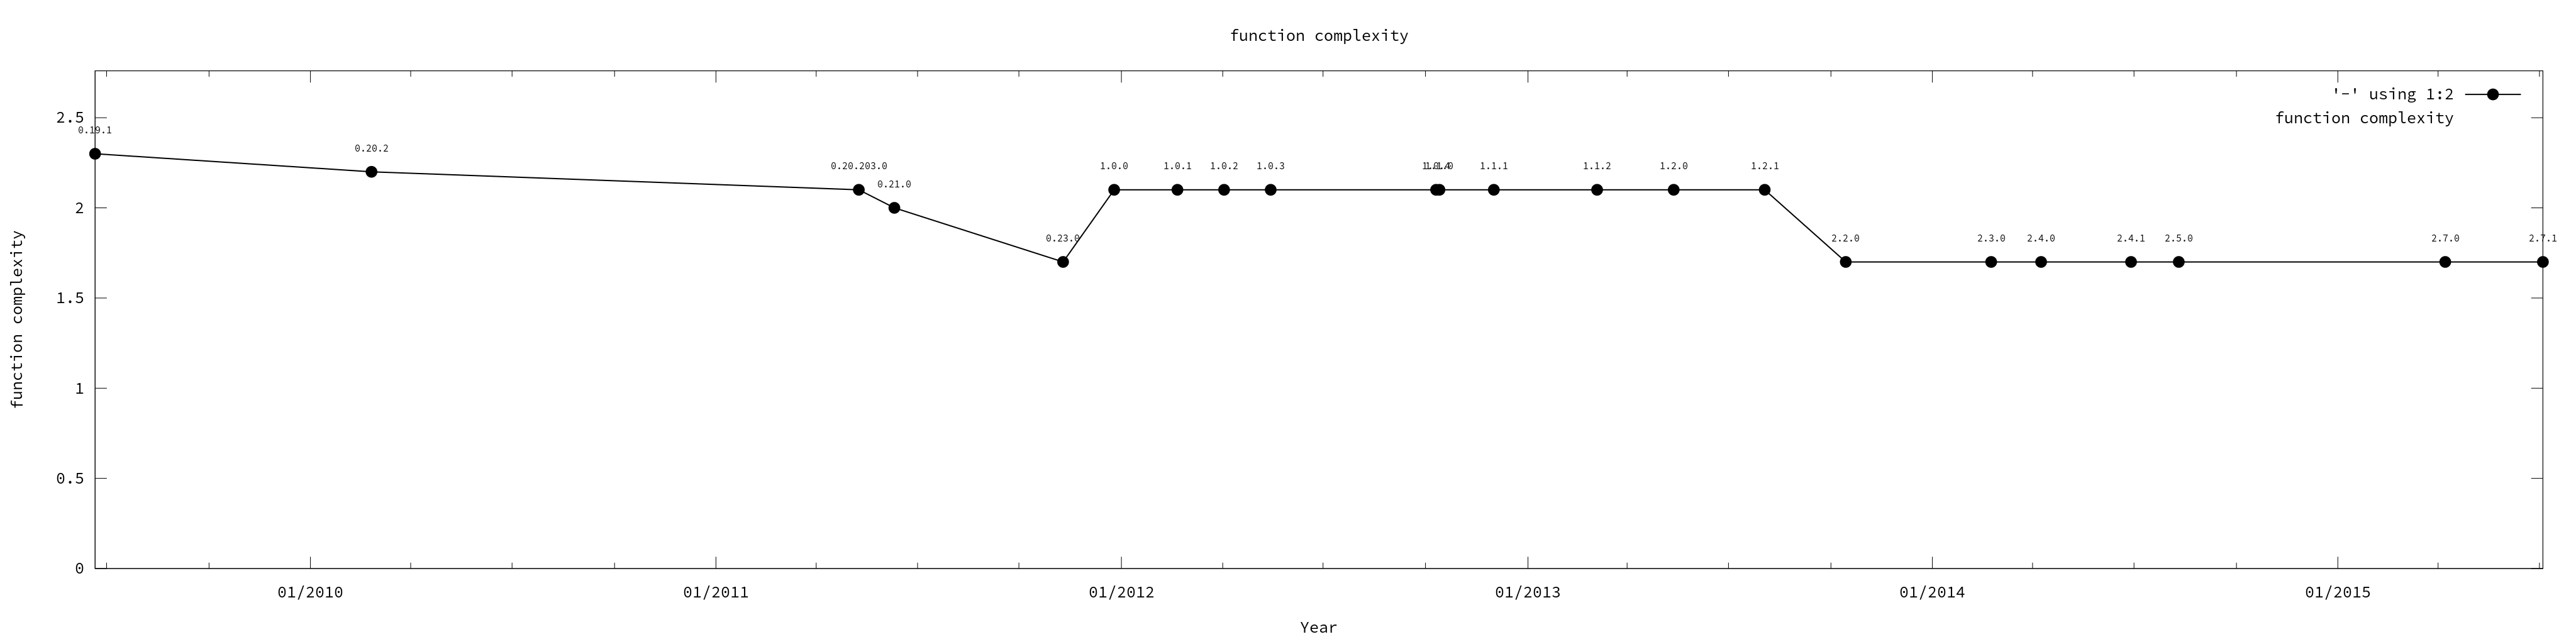
\includegraphics[width=1\linewidth]{figure/function_complexity}
	\caption{Evolução da complexidade ciclomática/Função}
	\label{fig:functioncomplexity}
\end{figure}
\begin{figure}[h]
	\centering
	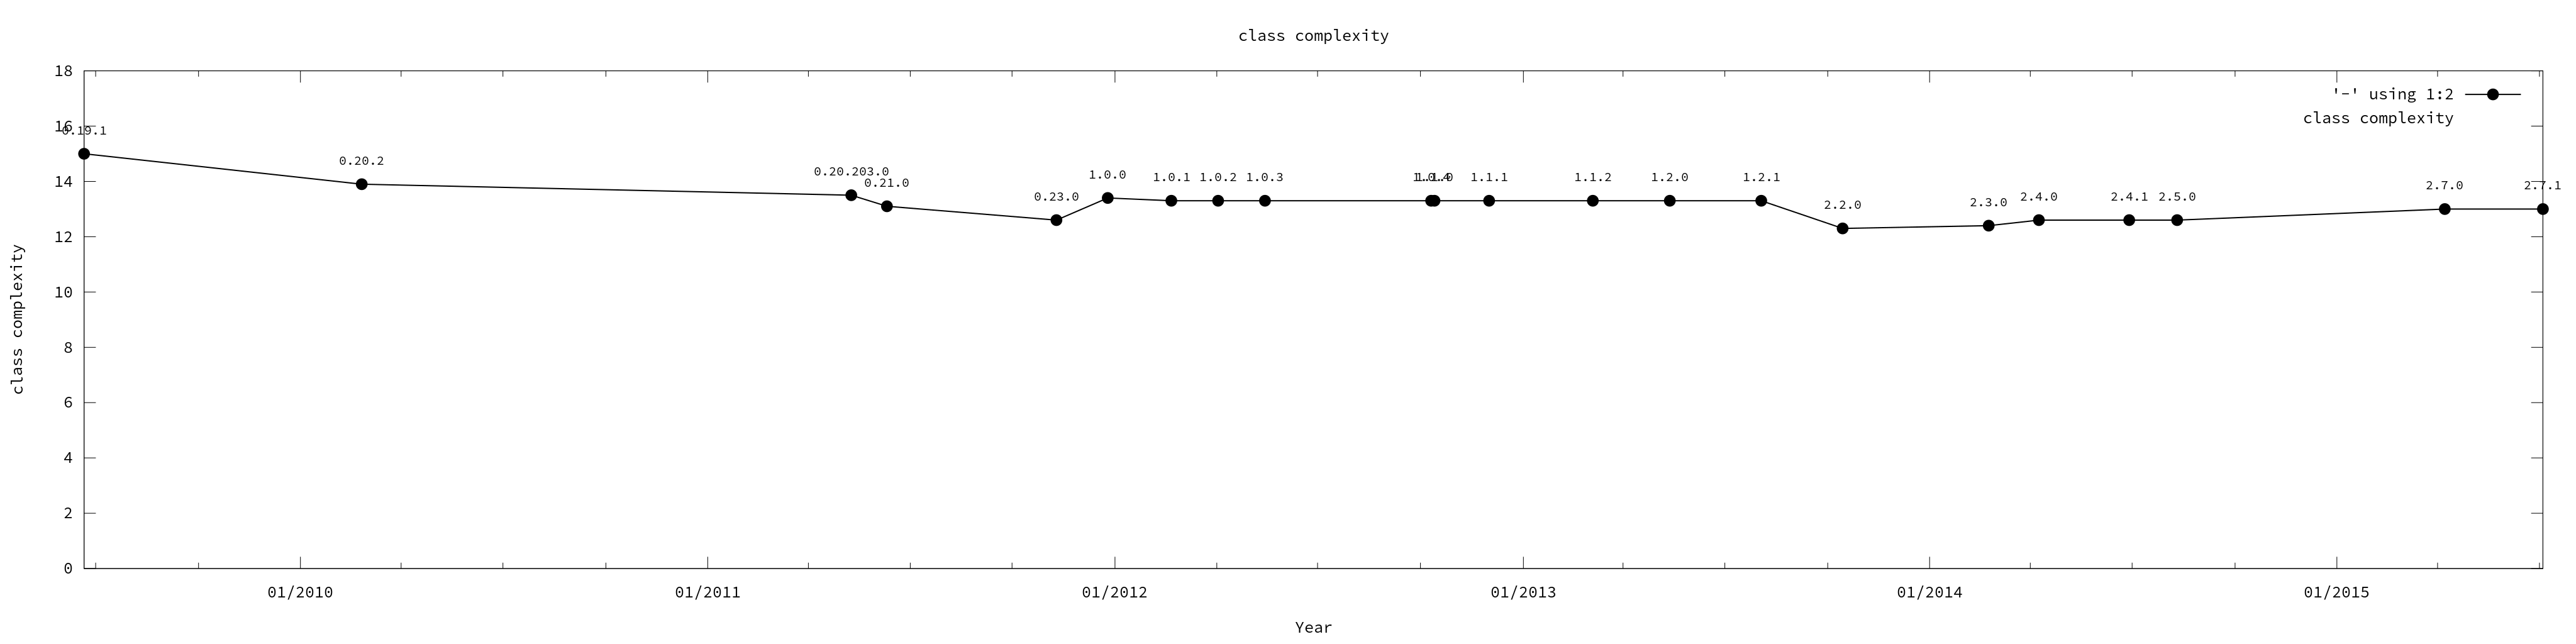
\includegraphics[width=1\linewidth]{figure/class_complexity}
	\caption{Evolução da complexidade ciclomática/Classe}
	\label{fig:classcomplexity}
\end{figure}

Em números absolutos, a complexidade cresce ao longo do tempo, o que esperado já que o projeto permanece em crescimento e a cada instrução adicionada existe uma complexidade básica associada, assim como apresentado na Seção \ref{subsec:complexidade_ciclomatica}. Os picos observados na Figura \ref{fig:total_complexity} acompanham o crescimento do projeto em geral.

Entretanto, considerando a complexidade do código relativa ao seu tamanho como nas Figuras \ref{fig:file_complexity}, \ref{fig:functioncomplexity}, \ref{fig:classcomplexity}, o projeto não aparenta tornar-se desproporcionalmente complexo ao longo de sua evolução, apresentando uma leve tendência à redução da complexidade relativa. Lehman argumenta que a complexidade aumenta ao longo do tempo, a não ser que esforço seja feito para conter seu avanço. Porém, não é evidente que na evolução do Hadoop houveram esforços focados no controle da condição, sugerindo que o projeto evolui com trabalho constante na amenização da complexidade.

Portanto, pode-se a afirmar que a Segunda Lei de Lehman não pode ser confirmada para o \textit{Hadoop}.

\subsection{Lei 3: Auto-Regulação}
Esta lei sugere que a evolução de um grande \textit{sistema} de \textit{software} é auto-regulado, ajustando seu tamanho ao longo do tempo apresentando adições positivas e negativas de tamanho. Assim, o \textit{software} deve apresentar tanto ajustes positivos, quanto negativos nas tendências de crescimento do \textit{software}. Como utilizado em \cite{neamtiu2013towards} verificamos o crescimento incremental de classes e funções no projeto. Portanto, nossas hipóteses são:
\begin{hypothesis}
	O número de lançamentos com ajustes negativos ao número de funções é diferente de zero.
\end{hypothesis}
\begin{hypothesis}
	O número de lançamentos com ajustes negativos ao número de classes é diferente de zero.
\end{hypothesis}

\begin{figure}[h]
	\centering
	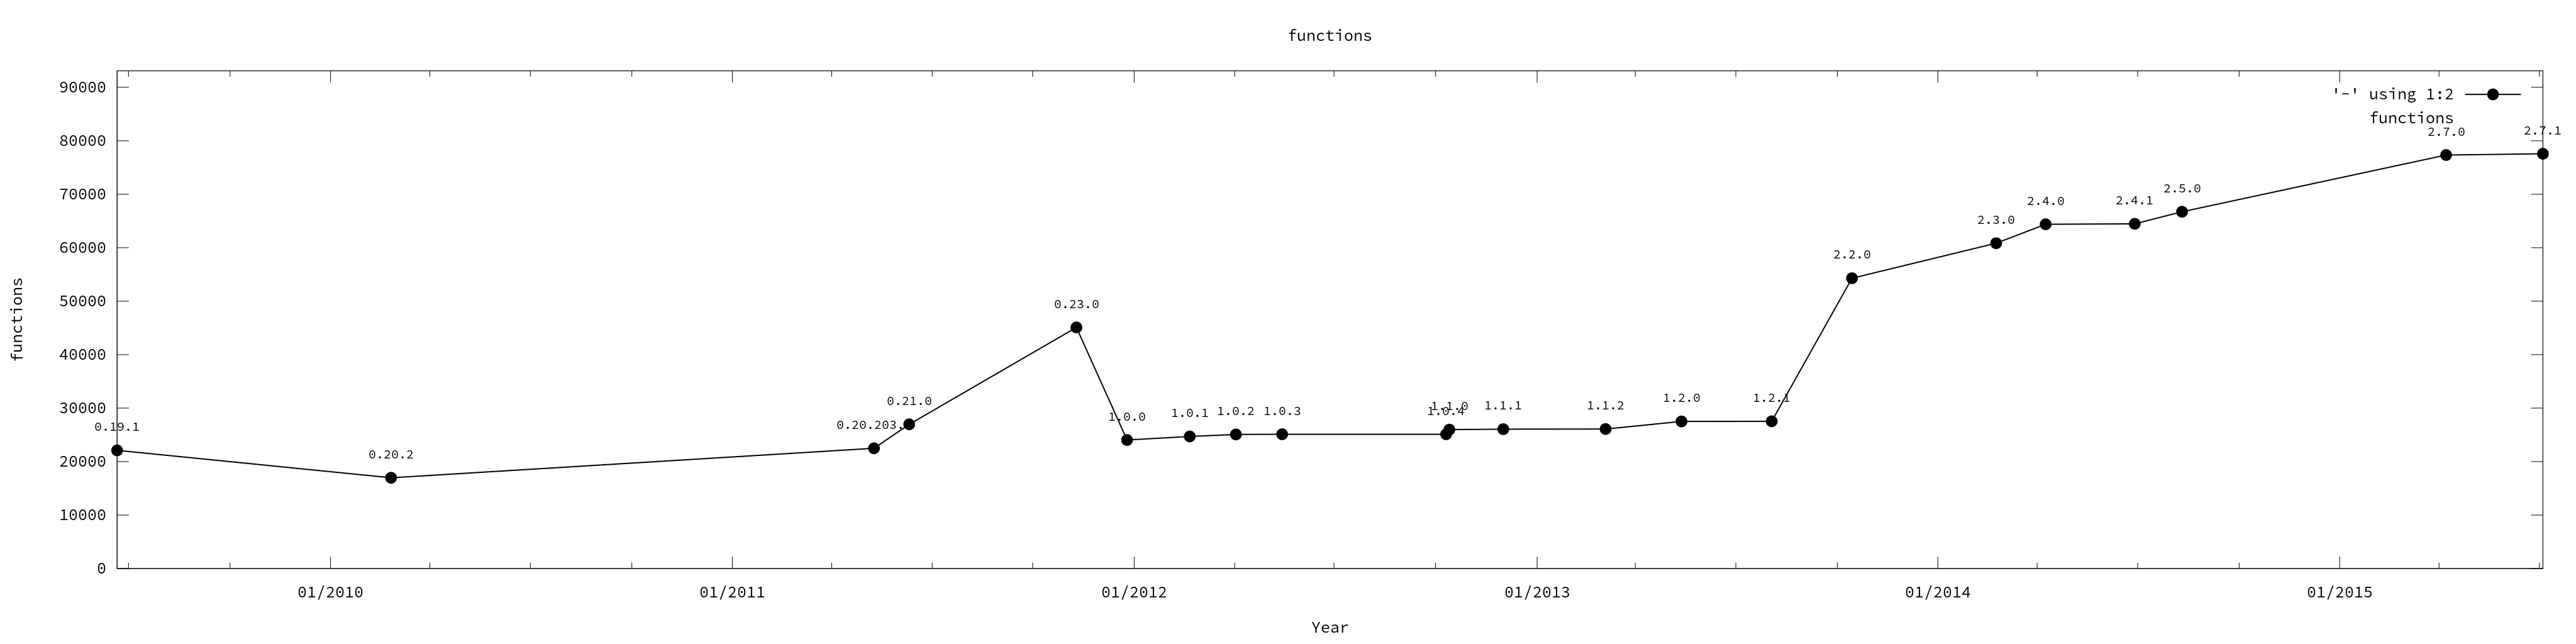
\includegraphics[width=1\linewidth]{figure/functions}
	\caption{Crescimento em número de funções}
	\label{fig:function_growth}
\end{figure}

\begin{figure}[h]
	\centering
	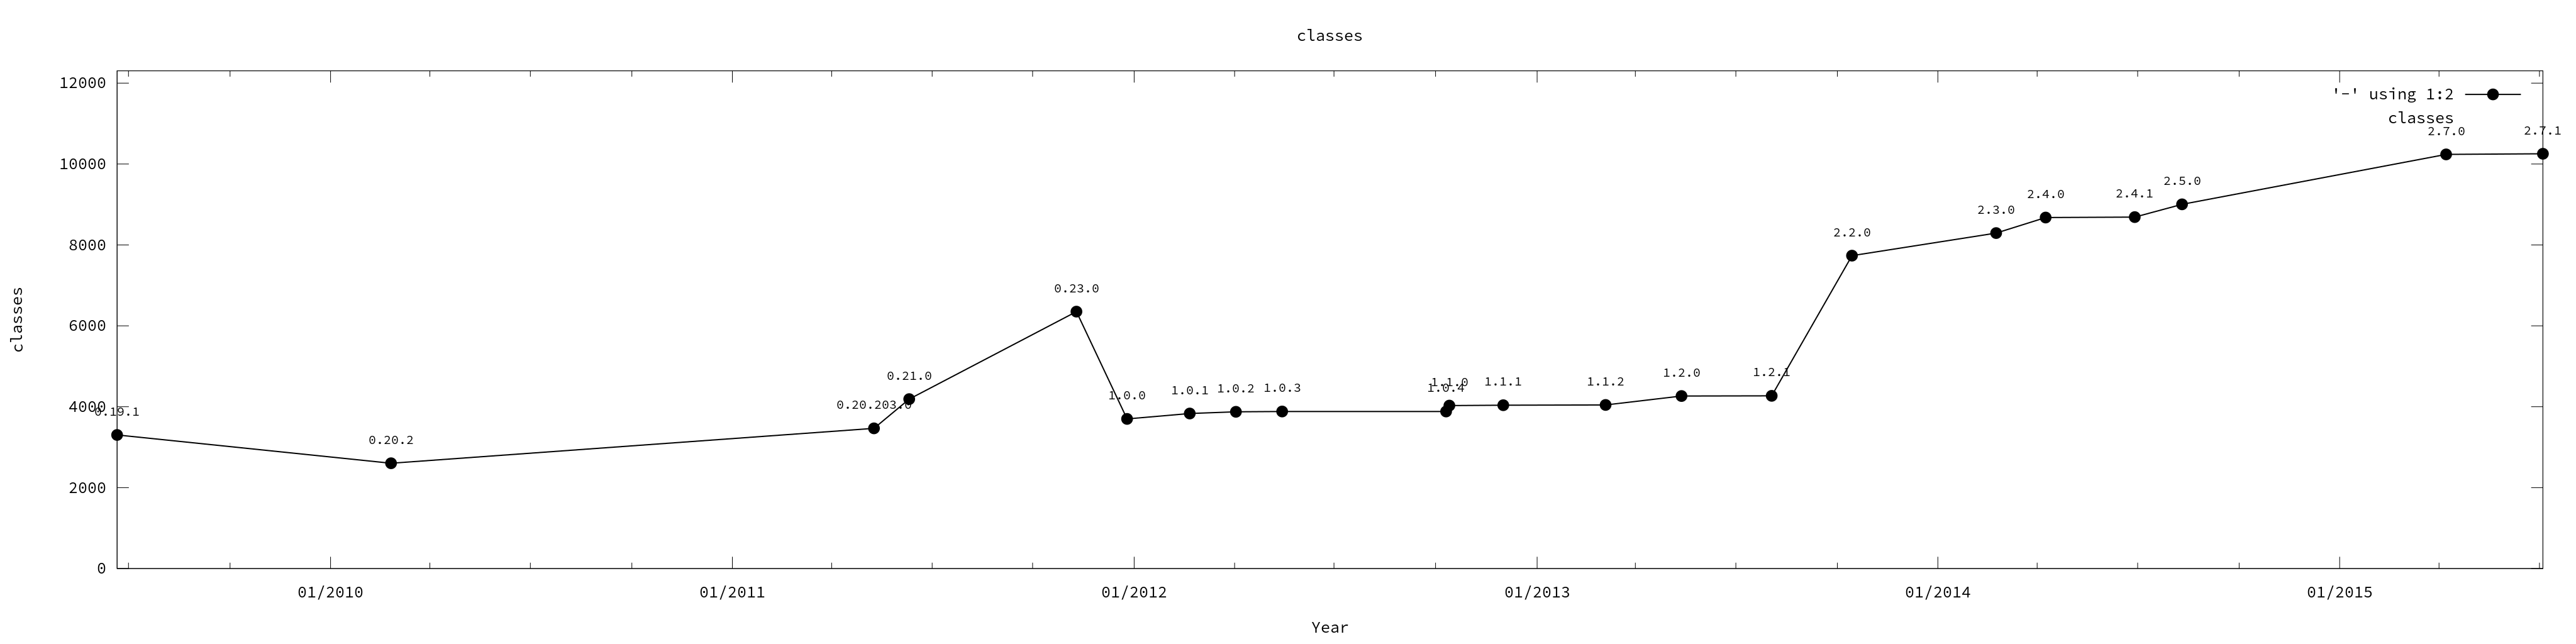
\includegraphics[width=1\linewidth]{figure/classes}
	\caption{Crescimento em número de classes}
	\label{fig:classes_growth}
\end{figure}

Nas Figuras \ref{fig:function_growth} e \ref{fig:classes_growth} pode-se representa o crescimento do número de funções e classes,  respectivamente. Pode-se observar que incrementos positivos são mais frequentes do que decrementos, mas ambos estão presentes.

Portanto, pode-se concluir que a Lei de Auto-Regulação é confirmada para o \textit{Hadoop}.


\subsection{Lei 4: Conservação da estabilidade Organizacional}
Esta lei, também conhecida como "taxa de trabalho invariante" estabelece que o ritmo de trabalho no ciclo de vida do software tende a permanecer constante durante a evolução do projeto. Como utilizado em \cite{neamtiu2013towards}, tomamos como definição de taxa de trabalho o número médio de mudanças realizadas por dia entre duas versões. Assim, nossas hipóteses são:
\begin{hypothesis}
	O número de médio de mudanças por dia é invariante.
\end{hypothesis}

\begin{hypothesis}
	O número de médio de mudanças por dia é invariante.
\end{hypothesis}
\begin{figure}
	\centering
	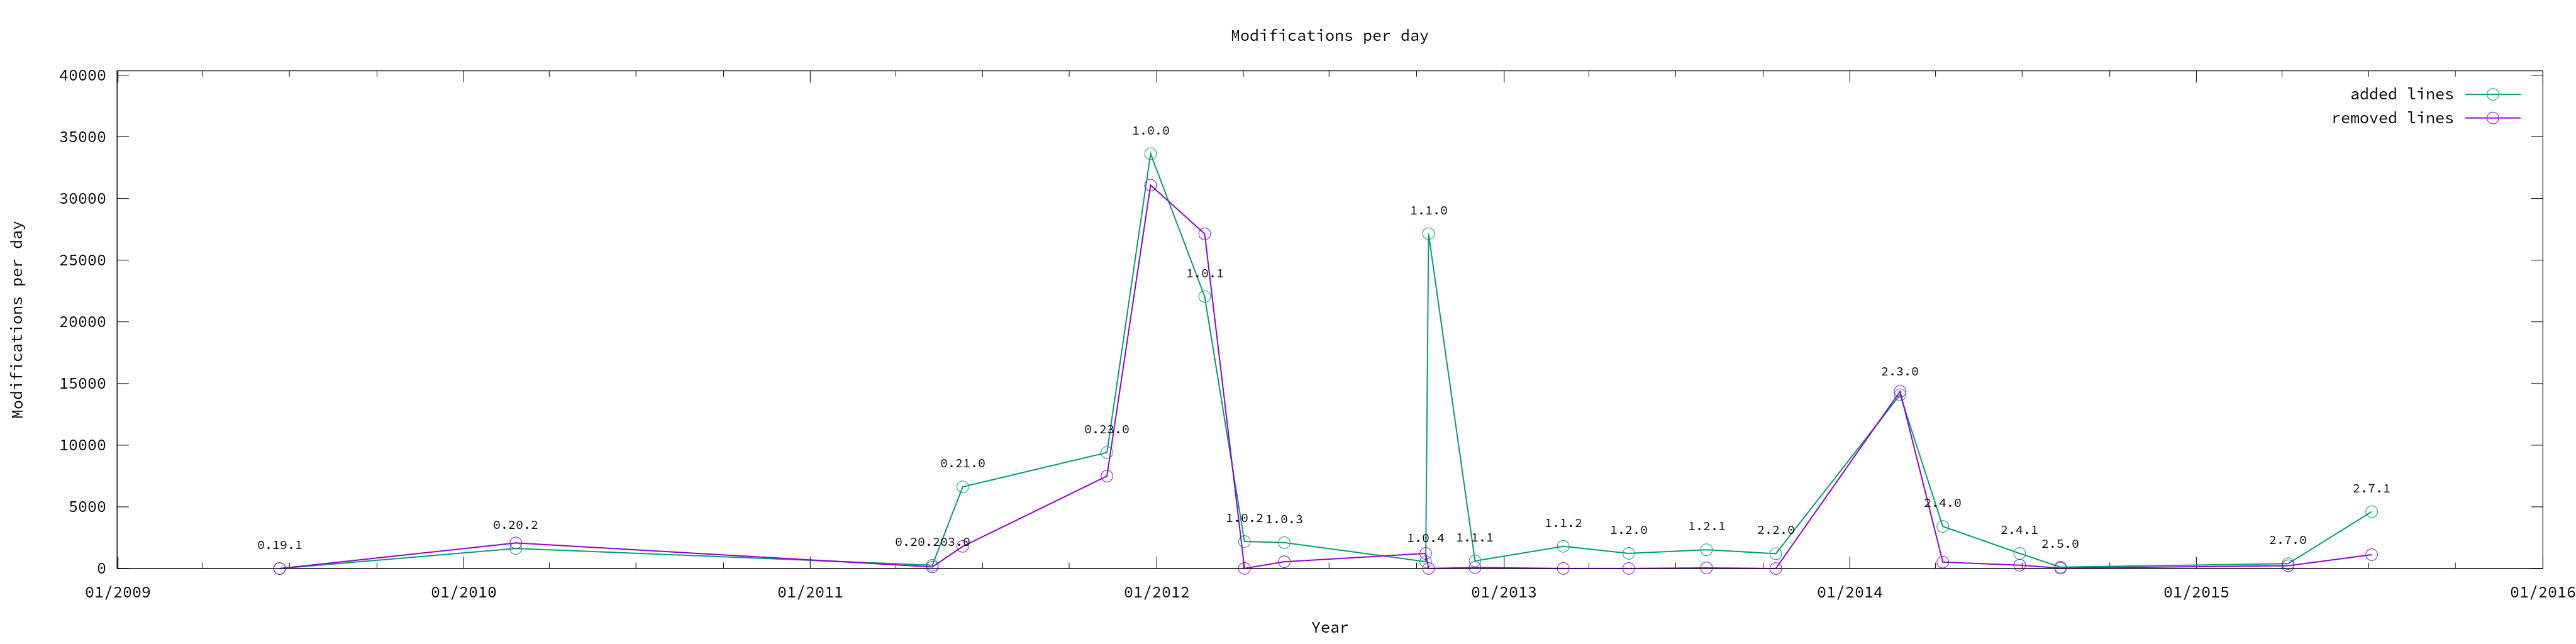
\includegraphics[width=1\linewidth]{figure/modifications_per_day}
	\caption{Média de modificações por dia}
	\label{fig:modificationsperday}
\end{figure}


A Figura \ref{fig:modificationsperday} mostra o número médio de adições e remoções por dia, calculados entre uma versão e sua antecessora. Nota-se que as maiores médias estão relacionadas mudanças de versões principais, como o grande taxa de trabalho para a versão 1.0.0, mas há também pontos onde uma grande quantidade de alterações foi feita em um pequeno espaço de tempo, como entre a versão 1.0.4 e 1.1.0. Pode-se observar também que não uma tendência a invariância, e sim uma grande variação das médias tanto do número de adições, quanto de remoção de linhas. O que não é surpreendente, em vista que se trata de um projeto Open-Source, em que não há um esforço igualmente investido por todos os desenvolvedores.

Portanto, verificamos que a lei da conservação da estabilidade organizacional é não é confirmada para o \textit{Hadoop}.
%\begin{hypothesis}
%	A taxa de mudança ao longo do tempo decresce.
%\end{hypothesis}
%\begin{hypothesis}
%	A taxa de crescimento ao longo do tempo decresce.
%\end{hypothesis}
\subsection{Lei 5: Conservação da Familiaridade}
Esta lei sugere que o crescimento incremental do sistema tende a permanecer constante, porque os desenvolvedores precisam entender o código fonte e o comportamento do sistema. Como métricas, utilizamos o incremento percentual de funções e classes por versão do projeto. Assim, nossas hipóteses são:

\begin{hypothesis}
	A taxa de crescimento de funções é invariante.
\end{hypothesis}
\begin{hypothesis}
	A taxa de crescimento de classes é invariante.
\end{hypothesis}
\begin{figure}[h]
	\centering
	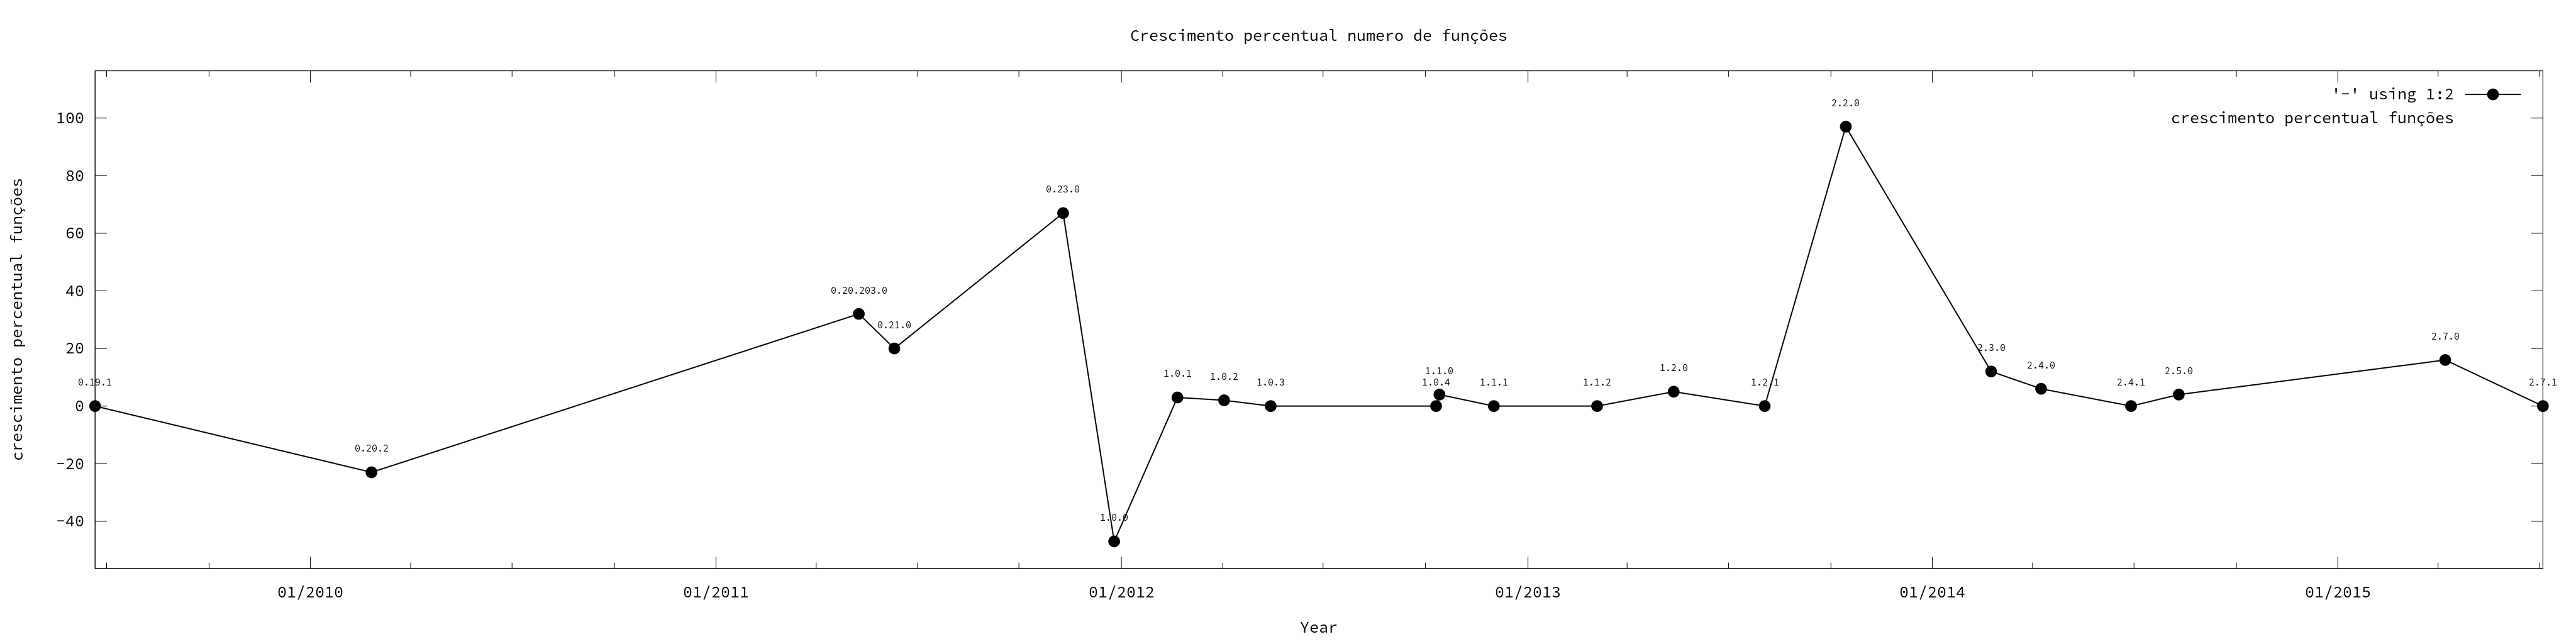
\includegraphics[width=1\linewidth]{figure/crescimento_percentual_funcoes}
	\caption{Crescimento percentual de funções por versão}
	\label{fig:crescimentopercentualfuncoes}
\end{figure}
\begin{figure}[h]
	\centering
	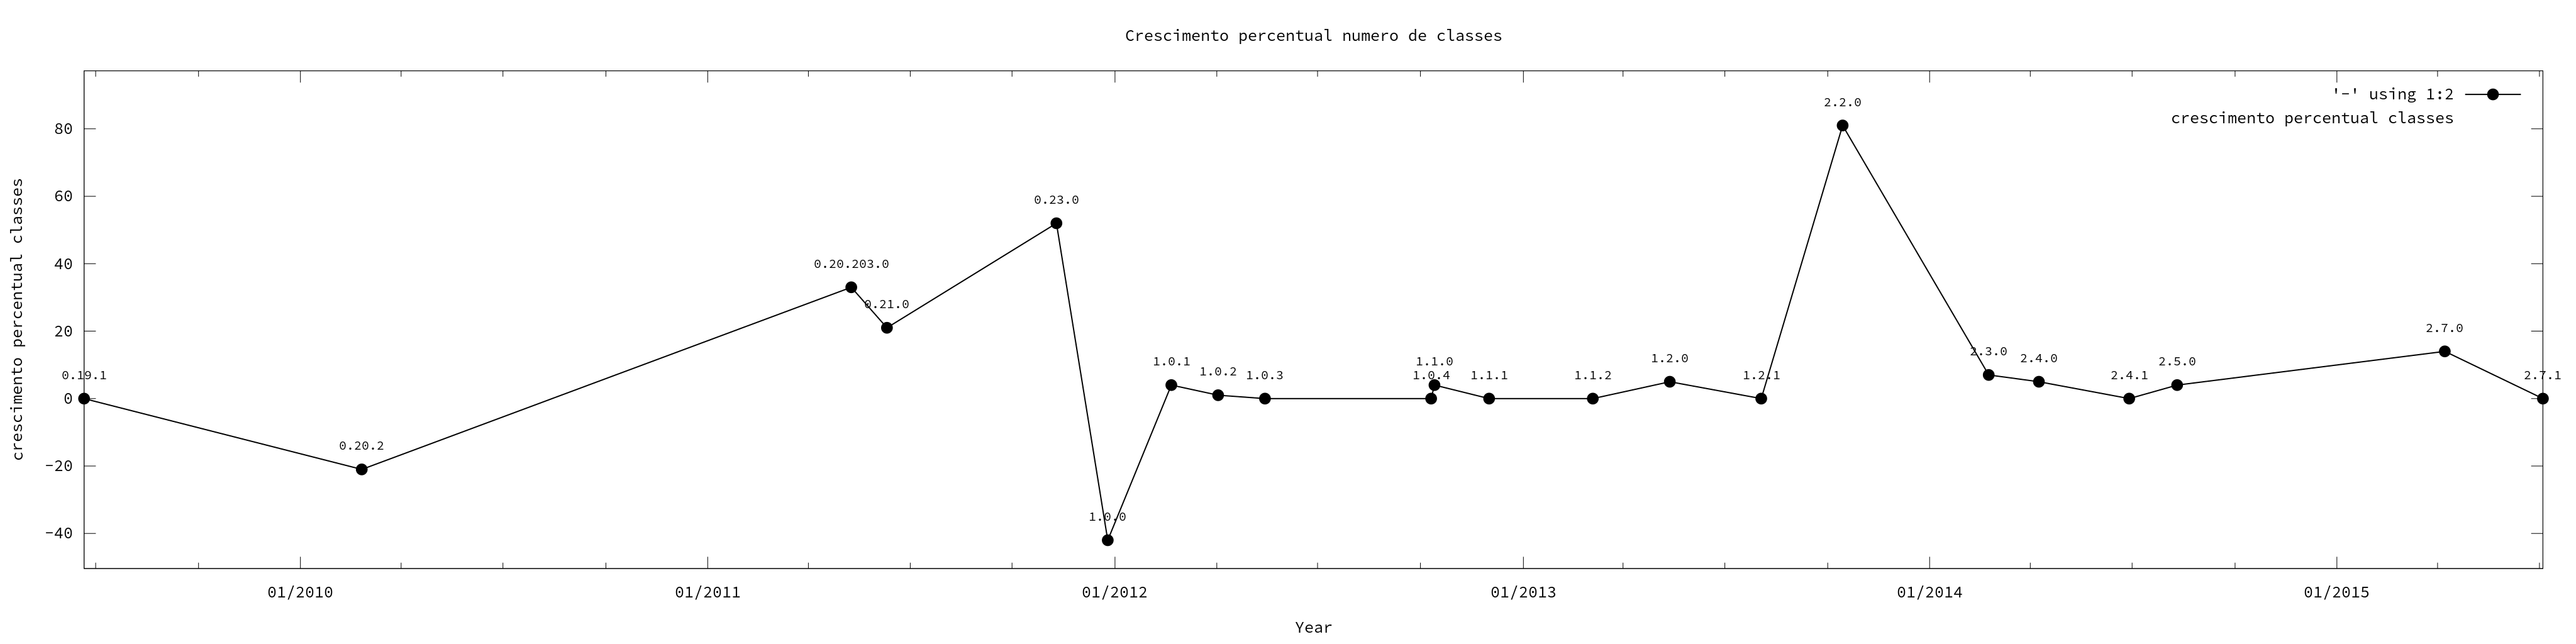
\includegraphics[width=1\linewidth]{figure/crescimento_percentual_classes}
	\caption{Crescimento percentual de classes por versão}
	\label{fig:crescimentopercentualclasses}
\end{figure}

As Figuras \ref{fig:crescimentopercentualfuncoes} e \ref{fig:crescimentopercentualclasses} representam o crescimento percentual de funções e classes, respectivamente. Assim como previsto em \cite{lehman1996laws}, versões que adicionam grandes mudanças são seguidas por lançamentos menores. Porém, ambos os indicadores mostram grande variação na adição de modificações, invalidando nossas hipóteses.

Portanto, a lei de conservação da familiaridade não pode ser confirmada para o \textit{Hadoop}.
\subsection{Lei 6: Crescimento Contínuo}
De acordo com esta lei, um sistema de \textit{software} deve ser constantemente incrementado ao longo do tempo para satisfazer usuários. Aqui, "crescimento" é interpretado como o tamanho do software. O tamanho pode também ser utilizado ou indicador de funcionalidade, assumindo-se que código adicional é escrito para a criação de novas funcionalidades.

Tal lei pode ser validada calculando métricas de tamanho (como número de módulos) e observando sua evolução com o tempo, assim como usado por Lehman e outros estudos\cite{lehman1980programs, lehman1985program,neamtiu2013towards}. Várias métricas podem ser utilizadas para descrever o tamanho de um software. Para o objeto de nossa análise, utilizamos linhas de código executáveis(isto é, não em branco e não comentadas), número de funções e classes para descrever o crescimento do projeto.
Portanto, nossas hipóteses são:
\begin{hypothesis}
	O número de linhas de código cresce com o tempo.
\end{hypothesis}
\begin{hypothesis}
	O número de classes cresce com o tempo.
\end{hypothesis}
\begin{hypothesis}
	O número de funções cresce com o tempo.
\end{hypothesis}

\begin{figure}
	\centering
	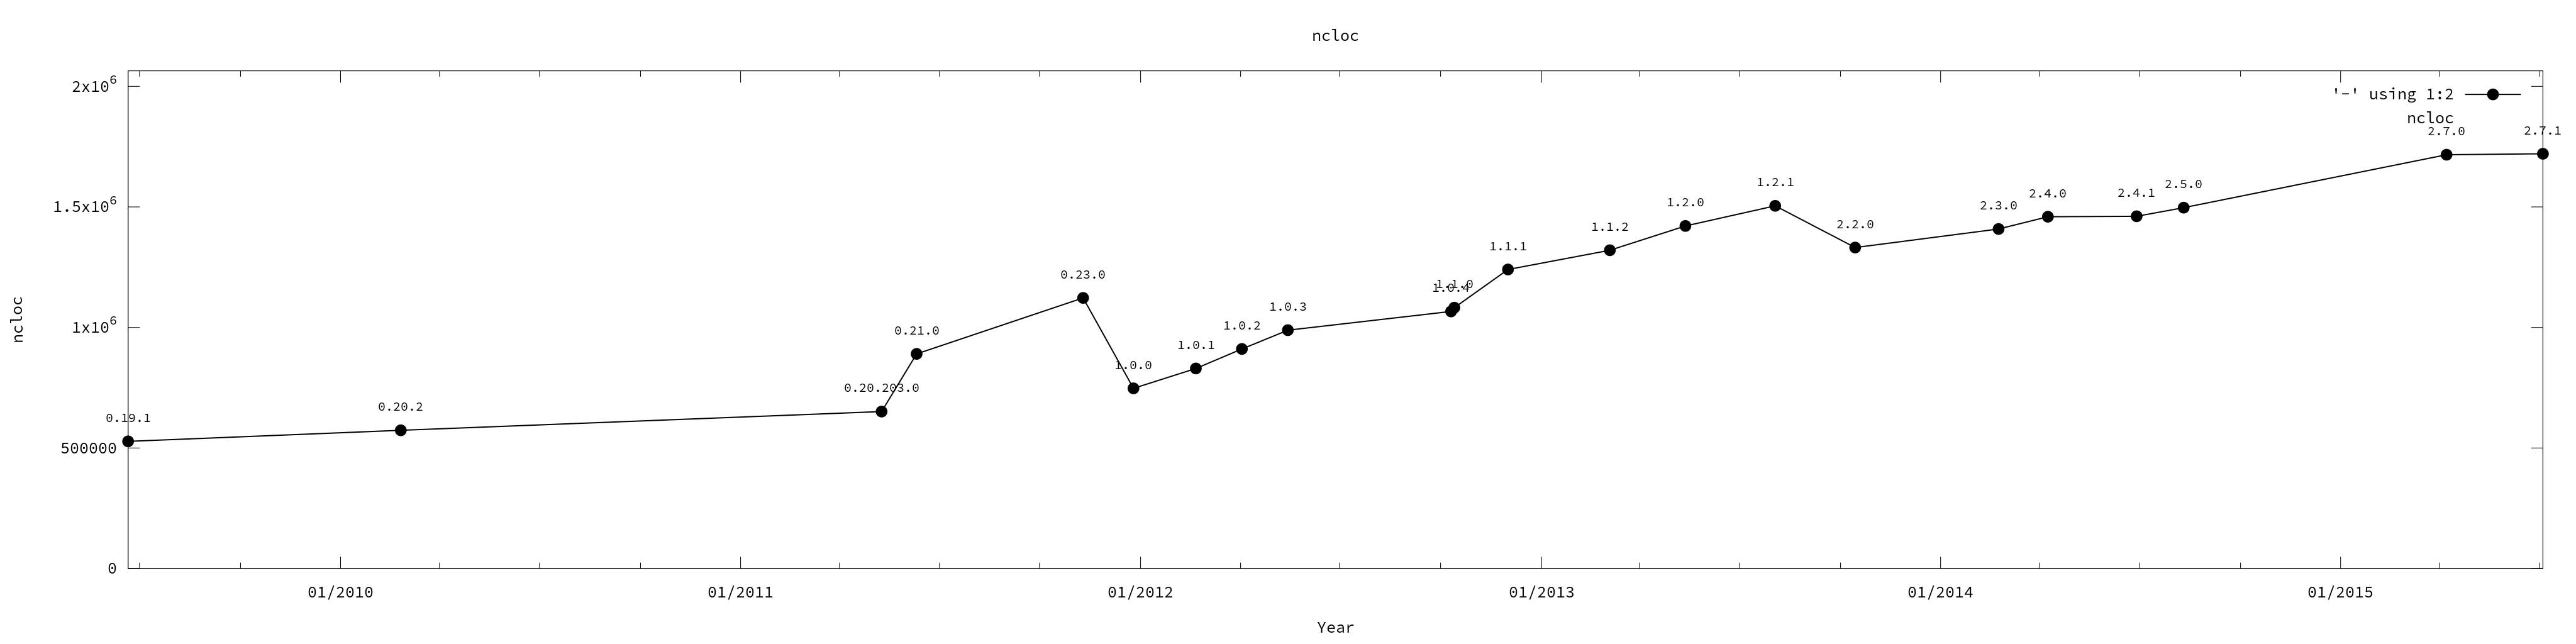
\includegraphics[width=1\linewidth]{figure/ncloc}
	\caption{Crescimento em Linhas}
	\label{fig:lines}
\end{figure}

As Figuras \ref{fig:function_growth}, \ref{fig:classes_growth} e \ref{fig:lines} mostram o crescimento em número de funções, classes e linhas de código, respectivamente. Com poucas exceções ao longo da sua evolução, observa-se que o Hadoop apresenta uma tendência de crescimento tomando toda seu histórico como referência, confirmando nossas hipóteses. 

Logo, podemos afirmar que a lei de crescimento contínuo é confirmada para o \textit{Hadoop}.

\subsection{Lei 7: Qualidade Decrescente}

Esta lei estipula que com o tempo, a qualidade do software parece degradar-se, a não ser que medidas sejam tomadas para conter tal fenômeno. Por qualidade de código, limitamos nossas observações a manutenibilidade de código em questão, mensurada através da dívida técnica do \textit{software}, como definida na Seção \ref{subsec:technical_debt}.
Assim, nossas hipóteses são:
\begin{hypothesis}
	A dívida técnica total cresce com o tempo.
\end{hypothesis}
\begin{hypothesis}
	A dívida técnica relativa total cresce com o tempo.
\end{hypothesis}
\begin{figure}[h]
	\centering
	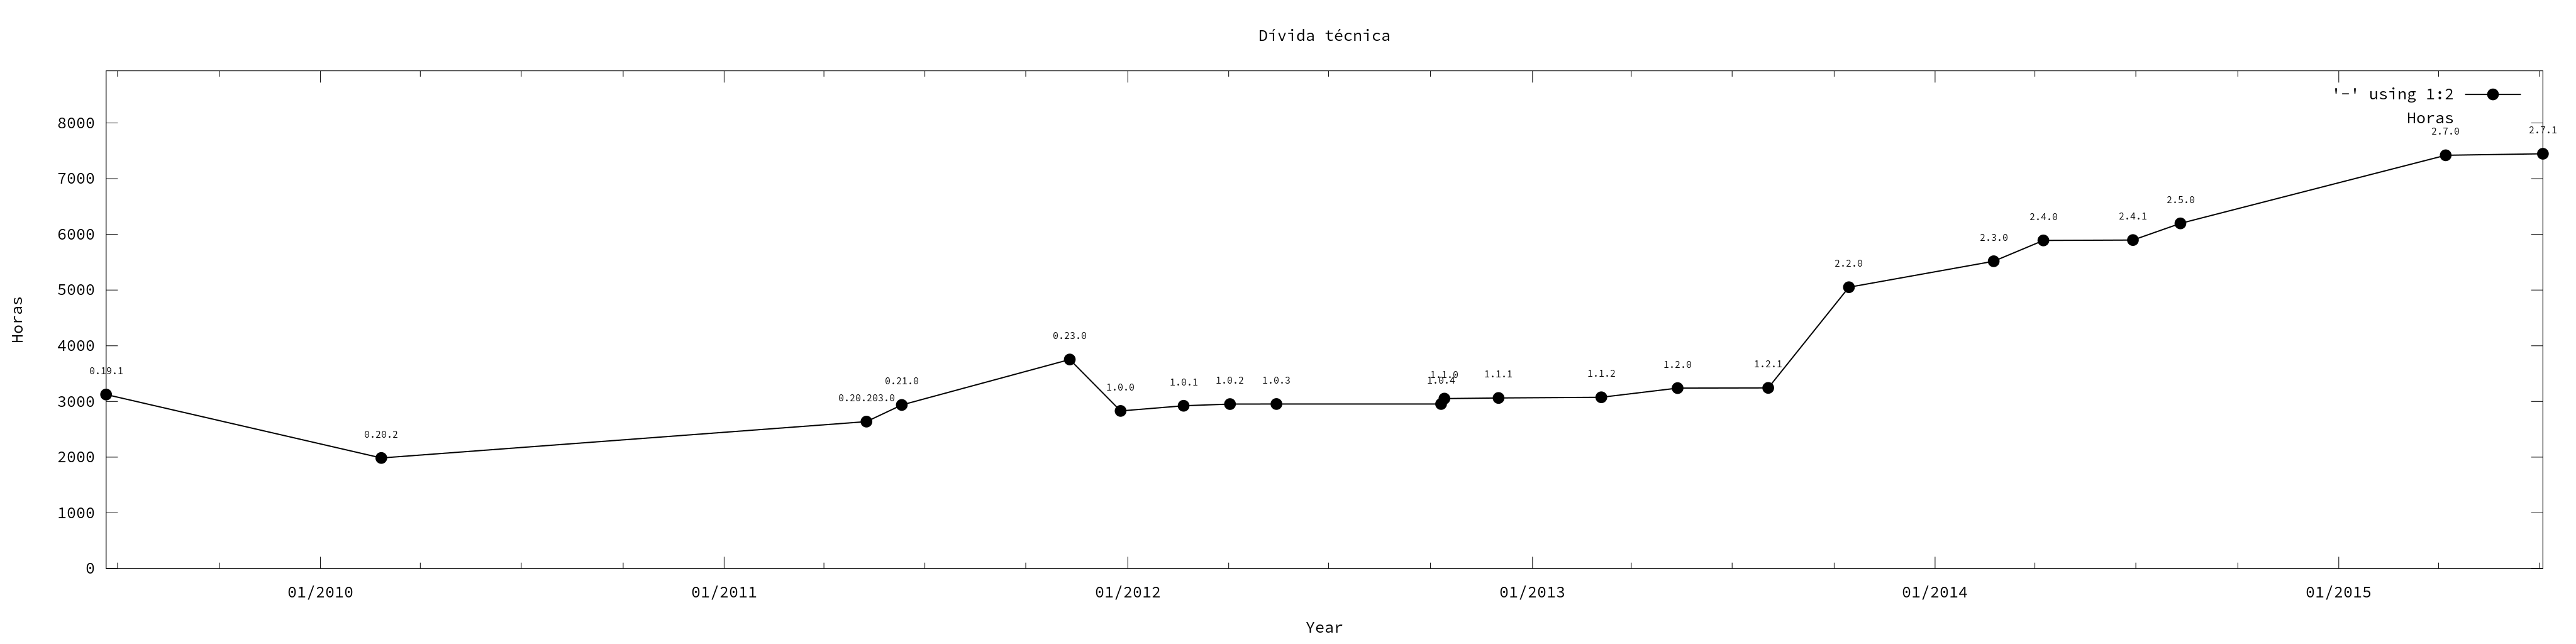
\includegraphics[width=1\linewidth]{figure/Horas}
	\caption{Dívida técnica total em horas}
	\label{fig:horas}
\end{figure}
\begin{figure}[h]
	\centering
	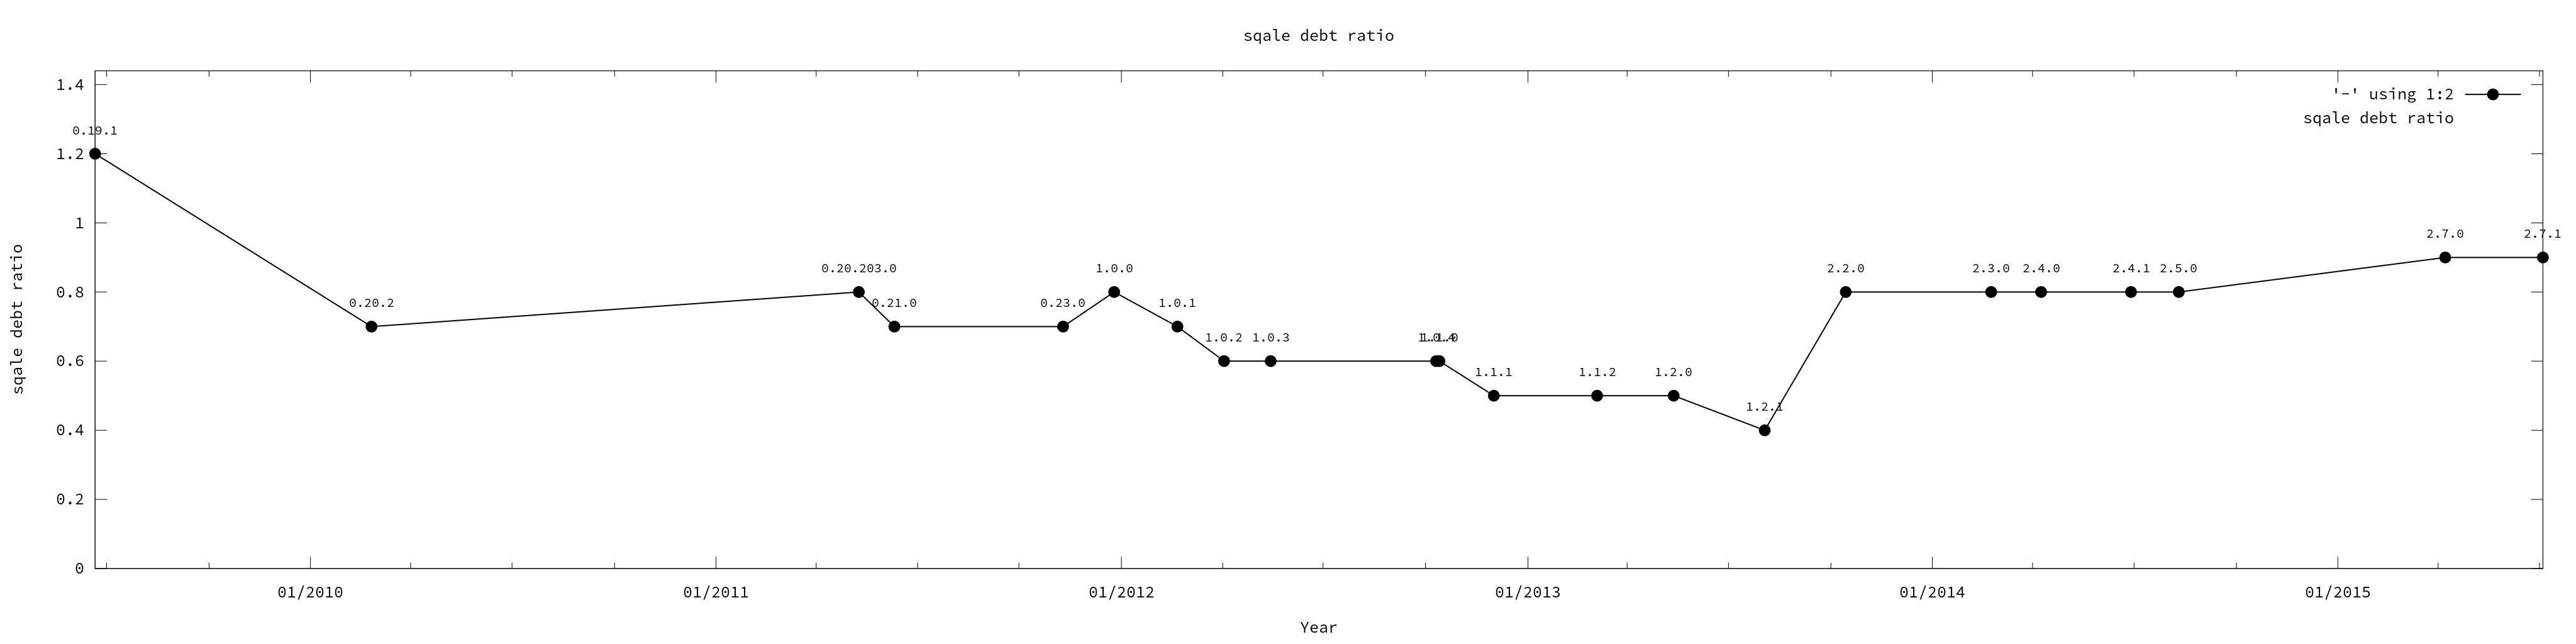
\includegraphics[width=1\linewidth]{figure/sqale_debt_ratio}
	\caption{Razão da dívida técnica}
	\label{fig:sqaledebtratio}
\end{figure}

Para a contabilização da dívida técnica, o \textit{Sonarqube} utiliza uma lista de regras que definem ocorrências de ``indesejáveis'' que caracterizam a dívida técnica no código, correção necessária e o tempo para adequar-lo a conformidade definida. Um exemplo de regras pode ser visto na Tabela \ref{table:Tabela de remediacao}. Para cada regra, descrita na coluna da esquerda, uma correção e tempo necessário para sua execução são definidos. Neste trabalho, foi utilizado o conjunto de regras padrão do \textit{Sonarqube} para a linguagem de programação Java, na qual o \textit{Hadoop} é escrito.

Para o cálculo da razão da dívida técnica, toma-se a razão entre o total da dívida técnica do projeto, sobre o esforço total para a recriação do projeto do zero, considerando o tempo para o desenvolvimento de uma linha de código igual a 30 minutos, padrão do \textit{Sonarqube}.
\begin{table}[h]
	\begin{centering}
		\begin{tabular}{|>{\centering}p{0.15\textheight}|c|>{\centering}p{0.1\textheight}|}
			\hline 
			Regra & Correção & Tempo para correção\tabularnewline
			\hline 
			\hline 
			Não há bloco de instrução comentado. & Remover, não há impacto no código compilado & 2 minutos por ocorrência\tabularnewline
			\hline 
			A indentação do código deve seguir uma padrão consistente & Ajustar com auxílio de recursos de IDEs & 2 minutos por ocorrência\tabularnewline
			\hline 
			Código deve sobrescrever tanto o método ``equals'' quanto ``hashcode'' & Escrever código e teste & 1h por ocorrência\tabularnewline
			\hline 
			Todos os arquivos possuem pelo menos 70\% de cobertura de testes & Escrever testes adicionais & 20 minutos por linha não não coberta para alcançar 70\% de cobertura\tabularnewline
			\hline 
			Não há trechos clonados de 100 palavras ou mais & Refatorar com IDE e escrever testes & 20 minutos por ocorrência\tabularnewline
			\hline 
		\end{tabular}
		\par\end{centering}
	\caption{Exemplo de Regras de Dívida Técnica}
	\label{table:Tabela de remediacao}
\end{table}


As Figuras \ref{fig:horas} e \ref{fig:sqaledebtratio} a dívida técnica total e a razão da dívida técnica, respectivamente. Pode-se observar no gráfico variações na dívida técnica total, que não acompanham o crescimento em total de linhas de código, apresentado na Figura \ref{fig:lines}, como, por exemplo, entre as versões 1.0.0 e 1.2.1, em que o número de linhas cresce consideravelmente, mas a dívida técnica total do projeto permanece relativamente constante, o que não acontece na transição da versão 1.2.1 para a 2.2.0, afetando consideravelmente a dívida técnica total, mesmo havendo uma redução do número de linhas de código total, demonstrando uma tendência de crescimento nas versões seguintes. 
Já a dívida técnica relativa, com exceção do período entre a versão 1.0.0 e 1.2.1, onde o baixo incremento da dívida técnica total e o aumento no total de linhas de código, parece permanecer constante. 
Desas forma, não podemos afirmar do ponto de vista da dívida técnica, que a qualidade de código parece deteriorar-se com o tempo.

Portanto, concluímos que a lei da qualidade decrescente não está confirmada para o \textit{Hadoop}.

\subsection{Lei 8: Sistema de Realimentação}

Assim como discutido em \cite{israeli2010linux}, o \textit{Hadoop} é sistema \textit{Open-Source} em que seu desenvolvimento é guiado pela comunidade de usuários. Como exemplos, temos relatórios de defeitos, correções e contribuições de novas funcionalidades feitas pela comunidade de usuários. Porém, não é claro como fazer a relação entre tais observações e uma medida quantitativa. 

Portanto, não apresentamos verificações para esta lei.

\section{Discussão}

Nesta seção, é apresentada uma revisão das observações realizadas neste trabalho. Na Tabela \ref{table:lawobservations}, são apresentadas as leis e suas respectivas observações neste trabalho. Pudemos encontrar evidências para sustentar nas Leis 1, 3, e 4, enquanto para as leis 2, 5 e 6 encontramos evidências do contrário. Porém, não podemos afirmar a invalidez destas leis devido às limitações do trabalho, descritos na Seção \ref{subsec:threadstovalidity}. Para um embasamento estatístico sólido, são necessários mais projetos em tipos diverssos de sistemas de \textit{software}.
\begin{table}[h]
	\begin{center}
		\begin{tabular}{|>{\centering}p{0.08\textwidth}|>{\centering}p{0.17\textwidth}|c|}
			\hline 
			Número & Lei de Lehman & Observação\tabularnewline
			\hline 
			\hline 
			1 & Mudança Contínua & Confirmada\tabularnewline
			\hline 
			2 & Complexidade crescente & Não confirmada\tabularnewline
			\hline 
			3 & Auto-Regulação & Confirmada\tabularnewline
			\hline 
			4 & Conservação da Estabilidade Organizacional & Não Confirmada\tabularnewline
			\hline 
			5 & Conservação da Familiaridade & Não Confirmada\tabularnewline
			\hline 
			6 & Crescimento contínuo & Confirmada\tabularnewline
			\hline 
			7 & Qualidade Descrescente & Não Confirmada\tabularnewline
			\hline 
			8 & Sistema de Realimentação & Não Avaliada\tabularnewline
			\hline 
		\end{tabular}
	\par\end{center}
	\caption{Observações das Leis de Lehman no Hadoop}
	\label{table:lawobservations}
\end{table}

Ainda assim, este trabalho demonstra como há grandes oportunidades em estudos de evolução de \textit{softwares Open-Source}, tendo em vista que o comportamento encontrado difere consideravelmente daquele encontrado em \cite{belady1976model,lehman1980programs,lehman1996laws}

\subsection{Ameaças a Validade} \label{subsec:threadstovalidity}
Esta seção aborda as possíveis ameaças a validade deste trabalho. As conclusões tiradas estão sujeitas a várias ameaças: validade de construção, validade de conteúdo, validade interna e validade externa.
\begin{itemize}
	\item \textbf{Validade de construção}: considera que as métricas utilizadas descrevem bem a característica desejada, por exemplo linhas de código, número de classes e número de funções descreverem bem o tamanho do sistema de \textit{software}. Várias métricas foram utilizadas com o objetivo de reduzir tal ameaça.
	\item \textbf{Validade de conteúdo}: assim como utilizado em \cite{neamtiu2013towards}, consideramos apenas lançamentos oficiais, e analisando o mair período possível da existência do \textit{Hadoop}. Considerar contribuições individualmente (\textit{commits}), ao invés de lançamentos oficiais pode comprometer a validade porque pode demonstrar ``ruídos'', como funcionalidades experimentais que acabam não sendo incluídas em lançamentos oficiais. Reconhecemos que algumas versões do início do \textit{Hadoop} não foram consideradas devido à falta de suas datas de lançamento do sistema de de controle de versão, o que pode afetar a validade do conteúdo.
	\item \textbf{Validade Interna}: depende da nossa capacidade de atribuir qualquer alteração nas caraterísticas do sistema como tamanho, por exemplo, ao tempo entre os lançamentos sem acidentalmente incluir ou excluir arquivos, classes ou outros. Tentamos mitigar tal possibilidade excluindo arquivos de configuração das análises do processamento, e limpando o diretório a cada novo lançamento.
	\item \textbf{Validade External}: a capacidade de generalizar os resultados para outros estudos. Também é ameaçada neste trabalho, já que tomamos apenas um projeto escrito em Java. Não podemos afirmar que os resultados são generalizáveis para sistemas proprietários ou sistemas de \textit{softare} escritos em outras linguagens.
\end{itemize}

